\documentclass[../CSC_52081_EP.tex]{subfiles}

\begin{document}
    \section{Introduction}
    \label{sec:intro}

Reinforcement Learning (RL) has become a powerful paradigm for developing autonomous agents that learn optimal behaviors through interactions with their environments. In this study, we employ the CarRacing-v3 environment provided by Gymnasium \cite{gymnasium}, which presents a challenging control task in a racing scenario. The environment is characterized by a high-dimensional observation space and two distinct modes for the action space. Specifically, the observation space consists of a top-down \(96\times96\) RGB image capturing both the car and the racetrack, thus requiring the use of deep convolutional neural networks (CNNs) for effective feature extraction.

\begin{figure}[H]
    \centering
    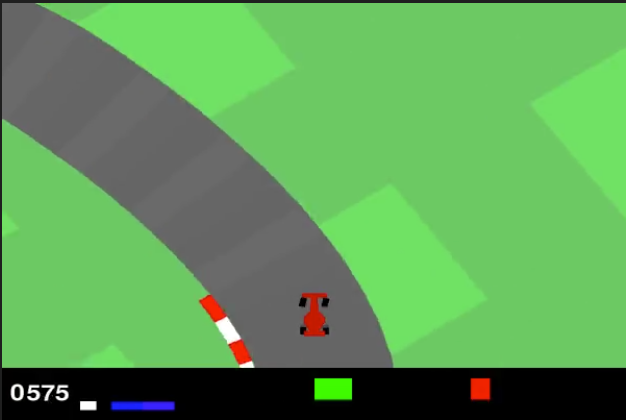
\includegraphics[scale = 0.3]{figures/car_racing_v3.png}
    \caption{A top-down 96x96 RGB image of the car and racetrack.}
    \label{fig:car_racing_v3}
\end{figure}

The primary objective of this project is to investigate and compare different RL policies across both discrete and continuous action modalities. For discrete action control, we implement methods such as Deep Q-Network (DQN) and SARSA. In contrast, for continuous action control, we explore approaches like the Cross-Entropy Method (CEM), and also incorporating policy gradient techniques (Proximal Policy Optimization (PPO) and Soft Actor-Critic (SAC)). This comparative analysis is driven by our interest in understanding the strengths and limitations of each method in handling complex decision spaces.

The dual nature of the action space in CarRacing-v3 presents a significant challenge. When dealing with high-dimensional visual inputs, the necessity of effective feature extraction becomes paramount. To address this, our approach includes the development of a convolutional neural network architecture tailored to process the \(96\times96\) RGB images, reducing their dimensionality while preserving essential spatial features required for decision making. Additionally, transitioning between discrete and continuous representations of actions requires careful algorithmic design and parameter tuning to ensure stable learning and convergence.

While previous studies have applied various RL techniques in simulated environments, many have tended to focus on either discrete or continuous action spaces separately. In our work, we adopt a comparative approach by evaluating different agents within the same CarRacing-v3 environment. This allows us to assess the performance of each method under similar conditions, examining aspects such as learning stability, computational complexity, and overall policy effectiveness.

The code for this project is available at \href{https://github.com/tr0fin0/ensta_CSC_52081_EP_project}{GitHub}.
\end{document}
